% MAVEB author manuscript
% Author-visible working version: clean paper rendering without review line numbers.
% For SIGGRAPH / SIGGRAPH Asia double-blind review, use:
% \documentclass[acmtog,anonymous,review]{acmart}
% \acmSubmissionID{paperID}
\documentclass[acmtog,nonacm]{acmart}

\usepackage{amsmath}
\usepackage{booktabs}
\usepackage{graphicx}
\usepackage{microtype}
\microtypesetup{expansion=false}
\usepackage[table]{xcolor}
\usepackage{tabularx}
\usepackage{array}
\usepackage{tikz}
\usetikzlibrary{arrows.meta,positioning,calc}

\setcopyright{none}
\settopmatter{printacmref=false,printfolios=true}
\renewcommand\footnotetextcopyrightpermission[1]{}

\newcommand{\method}{CBRC}
\newcommand{\system}{MAVEB}
\newcommand{\FULL}{\textsc{Full}}
\newcommand{\LOCAL}{\textsc{Local}}
\newcommand{\hard}{\textsc{Hard}}
\newcommand{\analytic}{\textsc{Analytic}}
\newcommand{\empirical}{\textsc{Empirical}}

\definecolor{mavebblue}{HTML}{D9E8FB}
\definecolor{mavebgreen}{HTML}{DFF1E1}
\definecolor{mavebamber}{HTML}{FBECC8}
\definecolor{mavebrose}{HTML}{F8DDE1}
\definecolor{mavebline}{HTML}{476582}
\newcommand{\tbhead}[1]{\textbf{#1}}
\newcolumntype{Y}{>{\raggedright\arraybackslash}X}
% Bounded tables: no implicit outer padding or unwrapped wide footnotes.
\setlength{\tabcolsep}{3pt}
\renewcommand{\arraystretch}{1.08}


\title{Repair What Matters: Criticality-Bounded Revision Cones for Persistent Captured Worlds}

\author{Swayam Singal}
\email{swayam.singal@gmail.com}
\renewcommand{\shortauthors}{Singal}
\emergencystretch=1em

\begin{abstract}
Persistent captured-world systems rarely contain geometry alone. Over time they collect observations, reconstruction state, explicit surface and appearance data, GPU-published records, and temporal rendering history. A physical change can be small in space and still reach much farther through this computational state. Restricting the update too aggressively risks leaving stale dependencies behind; rebuilding everything avoids that problem, but also throws away locality even when most of the world has no bearing on the output we care about.

We present \emph{Criticality-Bounded Revision Cones} (\method), implemented in \system. The framework is deliberately fail-closed: it uses regional recomputation only when the influence of the unrepaired exterior can be bounded for a stated quantity of interest. In practice, \method{} combines exact predecessor closure for structural dependencies with conservative finite-change bounds for the dependencies that admit them, then checks an explicit output-error contract and a frozen heterogeneous work model before allowing locality. Otherwise it returns \FULL{}. Every selected result is also replayed against an independent full-after reference, so the experiment checks the ordering measured full-reference error $\leq$ emitted bound $\leq$ declared tolerance rather than trusting the planner's own decision.

On the frozen public campaign, comprising 60 revisions over four RGB/SfM scenes, \method{} chose 44 certified-local repairs and 16 full rebuilds. We observed no certificate violation, and the native and reference planners agreed in all 60 cases. Importantly, 56 source edits were already above the protected RGB tolerance before repair, so the result is not explained by a collection of visually negligible edits. The calibrated work model gives a median selected work ratio of 0.36953 of \FULL{}, or 2.706$\times$ lower calibrated work. A separate five-case check on a pinned trained 3D Gaussian Splatting representation produced four local repairs, one fallback, and again no observed violation. The experiments also expose an unfinished part of the system: the frozen end-to-end path still inspects almost the entire Gaussian set. In isolation, exact sparse discovery reduces median inspection to 1\% without changing candidate selection. We therefore interpret the results as evidence for certified selective recomputation under the stated assumptions, not as a claim of universal safety, global optimality, or end-to-end wall-clock speedup.
\end{abstract}

\begin{CCSXML}
<ccs2012>
 <concept>
  <concept_id>10010147.10010371</concept_id>
  <concept_desc>Computing methodologies~Computer graphics</concept_desc>
  <concept_significance>500</concept_significance>
 </concept>
 <concept>
  <concept_id>10010147.10010371.10010396</concept_id>
  <concept_desc>Computing methodologies~Rendering</concept_desc>
  <concept_significance>500</concept_significance>
 </concept>
 <concept>
  <concept_id>10010147.10010371.10010352</concept_id>
  <concept_desc>Computing methodologies~Reconstruction</concept_desc>
  <concept_significance>300</concept_significance>
 </concept>
</ccs2012>
\end{CCSXML}
\ccsdesc[500]{Computing methodologies~Computer graphics}
\ccsdesc[500]{Computing methodologies~Rendering}
\ccsdesc[300]{Computing methodologies~Reconstruction}

\keywords{persistent captured worlds, incremental reconstruction, 3D Gaussian Splatting, certified recomputation, change-aware rendering, dependency analysis}

\begin{document}
\maketitle
\thispagestyle{plain}
\pagestyle{plain}
\raggedbottom

\section{Introduction}
Many 3D systems now live well beyond the capture session that created them. A reconstructed room may be revisited after furniture has moved; an AR map continues to exist while objects appear and disappear; a digital twin is updated after a small physical intervention. The stored state in these systems is not one uniform representation. Observations feed geometry, geometry determines surface or Gaussian support, materials and textures follow ownership and visibility, GPU records mirror persistent entities, and temporal filters reuse earlier screen-space state. For that reason, an edit that looks local in Euclidean space may not be local at all once it propagates through the system.

The safest response is still a global rebuild. Classical volumetric fusion and dense reconstruction give a natural full-reference notion of recomputation \citep{curless1996volumetric,newcombe2011kinectfusion,dai2017bundlefusion}. That choice is straightforward to reason about, but it becomes wasteful when only a small dependency closure is actually affected. Explicit scene representations make this mismatch particularly visible: large parts of a Gaussian map, or of a neural/hybrid reconstruction, may have no reason to change after a local revision \citep{kerbl2023gaussians,keetha2024splatam,matsuki2024monogs}. Continual Gaussian systems already exploit this fact by focusing optimization on changed regions or by managing stale observations over time \citep{ackermann2025clsplats,zeng2025gaussianupdate,yugay2026game}. Our concern is slightly different. Those systems mainly decide \emph{where to update}; here we ask how much error may safely remain outside the region that was chosen, across several kinds of derived state at once.

The systems question we focus on is deliberately narrow: \emph{when is it defensible to repair less than the whole captured world while still keeping an explicit output-error contract?} Reachability alone is not enough. Some relations are structural and, in our view, should not be approximated at all---ownership, record identity, publication, or an unstable temporal invalidation are examples. Other relations have finite influence that can be bounded from the implementation, such as the display-space effect of edited Gaussian support or a stable temporal blend. The revision policy therefore has to tell these cases apart. It must account for what is left outside a proposed repair region and fall back to a full rebuild when that remainder cannot be bounded tightly enough.

Our answer is \emph{Criticality-Bounded Revision Cones} (\method). A revision is represented on a typed dependency graph with three edge meanings. \hard{} edges carry exact structural requirements; \analytic{} edges carry conservative finite-change bounds; and \empirical{} edges may help decide what to try first, but they never become part of the safety certificate. For a proposed cone $C$, we certify the unrepaired exterior $O$ against the declared quantities of interest. The worst normalized certificate-to-tolerance ratio is the \emph{revision criticality}, with one as the decision boundary. We accept a local result only when exact predecessors are closed, every protected output is at or below that boundary, and the calibrated regional work is below the independently measured full baseline. If the coupling is unsupported, the residual is supercritical, the analytic assumptions are unstable, or locality simply costs too much, the planner returns \FULL{}.

\system{} implements this design as a C++23 persistent-world stack, alongside a dense Python reference certifier and an independent full-after Gaussian oracle. Figure~\ref{fig:overview} summarizes the decision path, while Figure~\ref{fig:poster} shows the support-selection idea visually. The implementation records immutable before/after revision sidecars, deterministic certificate JSON, per-domain work, and oracle replay. We do not treat the planner's own prediction as evidence that a repair is safe. Instead, the chosen result is replayed independently against \FULL{} and checked under the contract
\begin{equation}
E_q^{\mathrm{full-ref}} \le B_q(C) \le \varepsilon_q,
\label{eq:contract}
\end{equation}
where $E_q^{\mathrm{full-ref}}$ is the measured discrepancy from an independent full-after reference, $B_q(C)$ is the emitted conservative bound, and $\varepsilon_q$ is the declared tolerance for quantity of interest $q$.

We froze the protocol and the claim boundaries before reading the final campaign as evidence. On the 60 public RGB/SfM revisions, \method{} makes 44 certified-local selections and 16 automatic full rebuilds. We observed no certificate violation, and the native and Python planners made the same decision in every case. Also, 56 of the 60 source edits were above the protected RGB tolerance before repair, which matters: otherwise a zero post-repair residual could come from edits that were effectively irrelevant to begin with. The frozen millisecond calibration gives a median heterogeneous work ratio of 0.36953 of \FULL{}, corresponding to 2.706$\times$ lower calibrated work. We keep that wording deliberately---it is a work result, not a paired wall-clock speedup. On the pinned trained 3DGS representation, four of five revisions are local and one falls back, again with no observed violation. That experiment also makes the main implementation weakness hard to ignore: candidate discovery still behaves almost globally in the frozen end-to-end path.

The contributions are:
\begin{itemize}
    \item a fail-closed revision formulation for heterogeneous persistent captured worlds that combines exact dependency closure with conservative finite-change propagation;
    \item quantity-of-interest certification for local repair, including implementation-backed Gaussian display-space and stable temporal bounds, with unsupported dependencies retained as exact;
    \item a native work-aware revision planner with automatic \FULL{} fallback, deterministic evidence emission, a dense reference implementation, and independent full-after falsification; and
    \item frozen public and trained-representation evidence that reports local/full crossover, calibrated work, sparse-discovery behavior, negative or neutral ablations, and measured limitations without converting work reduction into speedup claims.
\end{itemize}

\begin{figure*}[t]
  \centering
  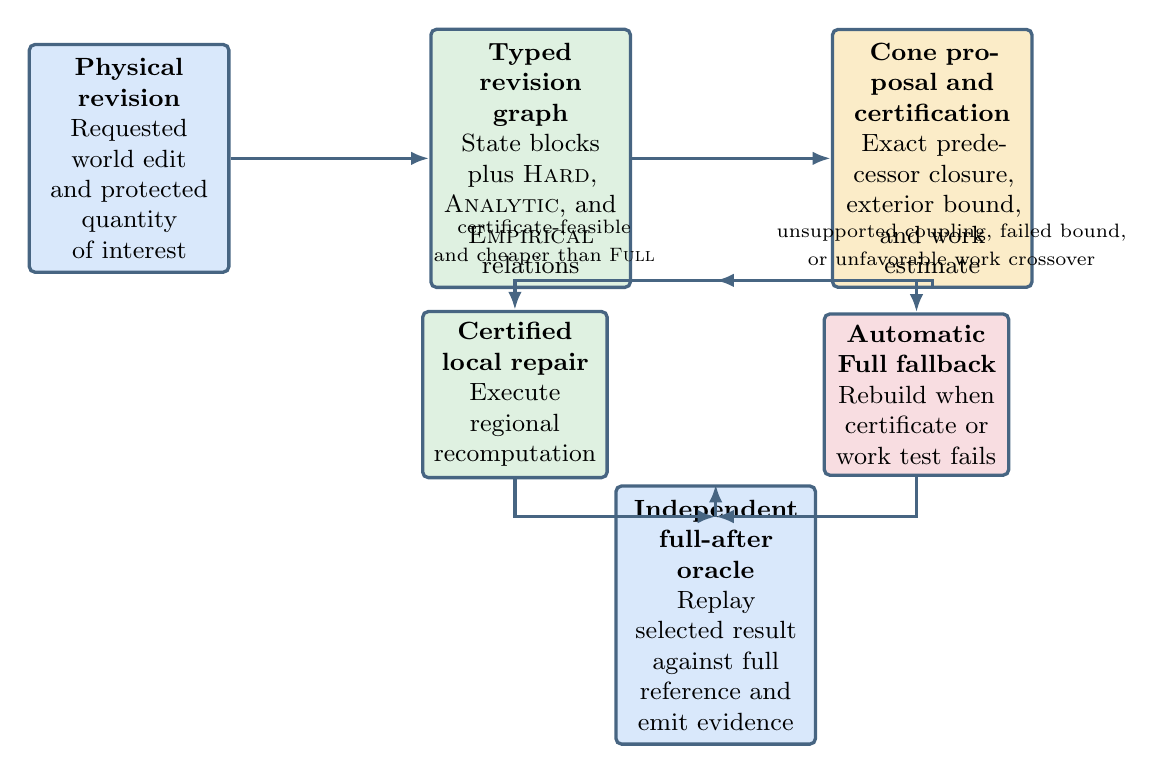
\begin{tikzpicture}[
  font=\small,
  box/.style={draw=mavebline, rounded corners=2pt, very thick, align=center,
              minimum height=10mm, text width=0.18\textwidth, inner sep=5pt},
  smallbox/.style={draw=mavebline, rounded corners=2pt, very thick, align=center,
                   minimum height=9mm, text width=0.17\textwidth, inner sep=4pt},
  arr/.style={-{Latex[length=2.3mm]}, very thick, draw=mavebline}
]
\node[box, fill=mavebblue] (revision) at (0,0)
  {\tbhead{Physical revision}\\Requested world edit and protected quantity of interest};
\node[box, fill=mavebgreen] (graph) at (5.1,0)
  {\tbhead{Typed revision graph}\\State blocks plus \hard{}, \analytic{}, and \empirical{} relations};
\node[box, fill=mavebamber] (cert) at (10.2,0)
  {\tbhead{Cone proposal and certification}\\Exact predecessor closure, exterior bound, and work estimate};
\node[smallbox, fill=mavebgreen] (local) at (4.9,-3.0)
  {\tbhead{Certified local repair}\\Execute regional recomputation};
\node[smallbox, fill=mavebrose] (full) at (10.0,-3.0)
  {\tbhead{Automatic \FULL{} fallback}\\Rebuild when certificate or work test fails};
\node[box, fill=mavebblue] (oracle) at (7.45,-5.8)
  {\tbhead{Independent full-after oracle}\\Replay selected result against full reference and emit evidence};
\draw[arr] (revision.east) -- (graph.west);
\draw[arr] (graph.east) -- (cert.west);
\coordinate (split) at (7.45,-1.55);
\draw[arr] (cert.south) -- (10.2,-1.55) -- (split);
\draw[arr] (split) -- (4.9,-1.55) -- (local.north);
\draw[arr] (split) -- (10.0,-1.55) -- (full.north);
\node[align=center, anchor=south east] at (6.8,-1.48)
  {\scriptsize certificate-feasible\\[-1pt]\scriptsize and cheaper than \FULL{}};
\node[align=center, anchor=south west] at (8.1,-1.48)
  {\scriptsize unsupported coupling, failed bound,\\[-1pt]\scriptsize or unfavorable work crossover};
\coordinate (merge) at (7.45,-4.55);
\draw[arr] (local.south) -- (4.9,-4.55) -- (merge);
\draw[arr] (full.south) -- (10.0,-4.55) -- (merge);
\draw[arr] (merge) -- (oracle.north);
\end{tikzpicture}

  \Description{Color boxed system architecture diagram for the CBRC decision and falsification path. A physical revision enters a typed graph, proceeds to cone proposal and certification, branches to certified local repair or automatic full fallback, and both branches go to an independent full-after oracle. Orthogonal arrows route around the boxes.}
  \caption{\method{} decision and falsification path. A physical revision enters a typed dependency graph. Exact \hard{} predecessors are closed, conservative \analytic{} influence is propagated to the unrepaired exterior, and quantity-of-interest bounds are checked against tolerance. A local repair is executed only when it is certified and cheaper than the full baseline; otherwise the system falls back to \FULL{}. The selected result is then replayed against an independent full-after oracle.}
  \label{fig:overview}
\end{figure*}

\begin{figure*}[t]
  \centering
  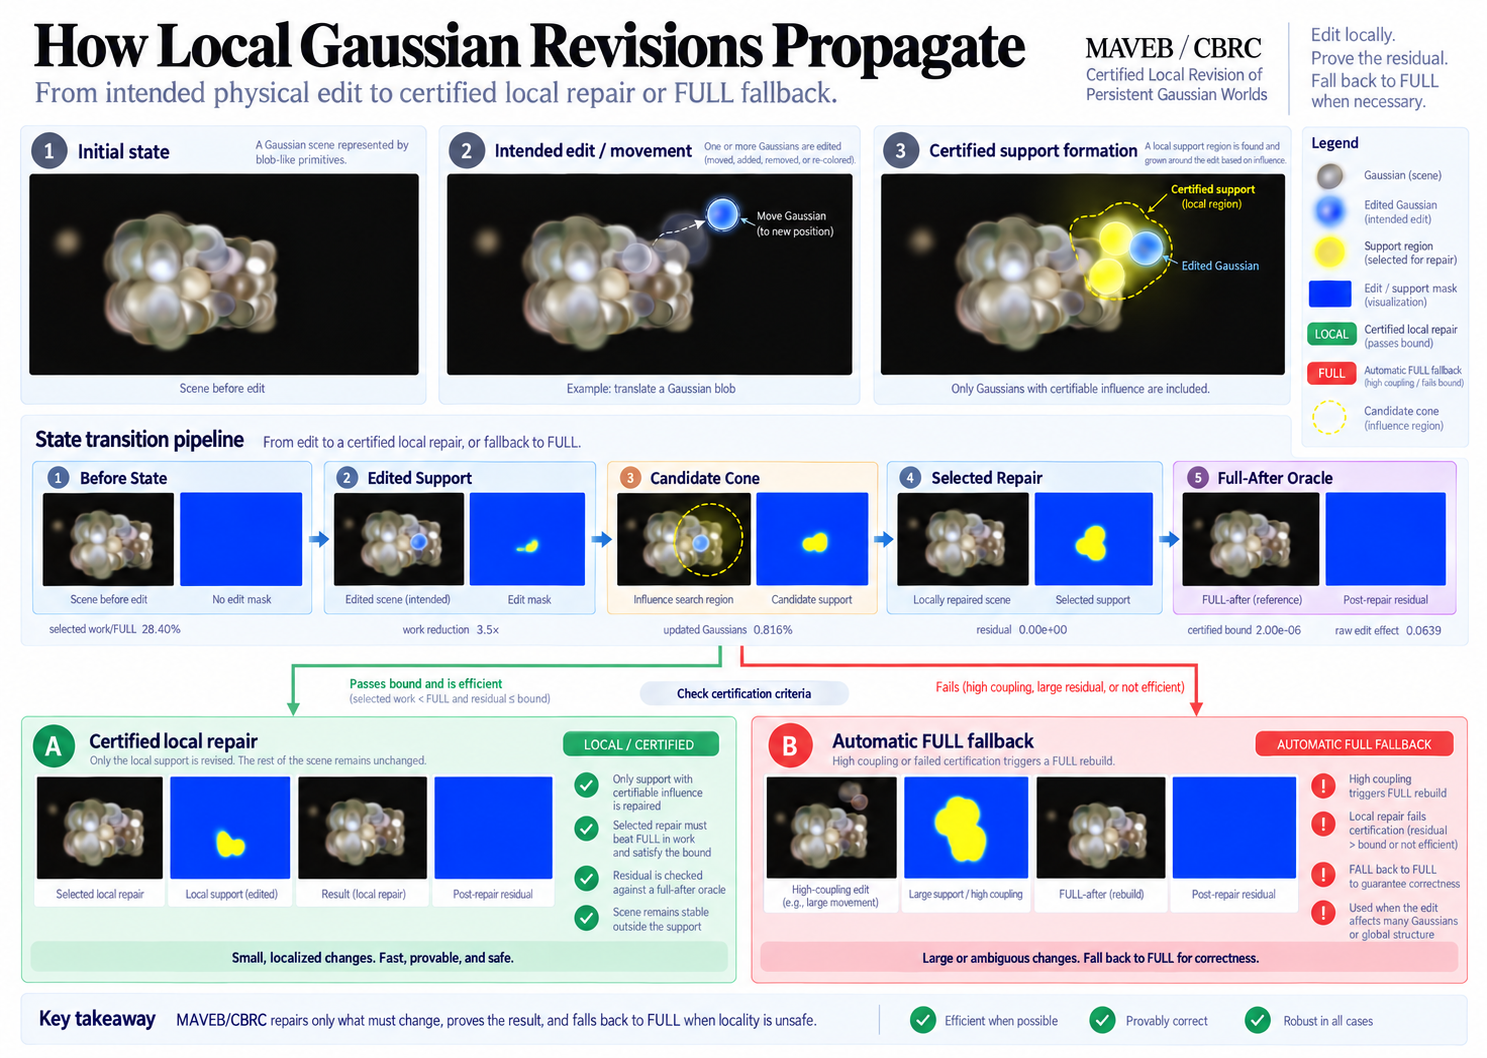
\includegraphics[width=\textwidth]{figures/figure2_exact.png}
  \Description{Author-supplied visual explanation of how a local Gaussian revision propagates through MAVEB/CBRC. The figure shows an initial Gaussian scene, an intended edited Gaussian, conservative certified support formation, a five-stage state-transition pipeline, and the two fail-closed outcomes: certified local repair or automatic full rebuild. Blue denotes intended edit state, yellow denotes selected repair support, green denotes a certified local outcome, and red denotes full fallback.}
  \caption{How a physical edit becomes a certified revision. An intended Gaussian edit induces a candidate influence region from which \method{} selects the support that must be repaired. Exact structural dependencies remain closed and the unrepaired exterior is accepted only when its quantity-of-interest bound satisfies the declared tolerance and regional work remains below the frozen \FULL{} baseline. The system therefore either revises only the certified support (A) or fails closed to a \FULL{} rebuild (B). Blue marks the intended edit, yellow the selected repair support. The supplied image is reproduced unchanged. Its 28.40\% work ratio, 3.5$\times$ work reduction, and other embedded micro-metrics are illustrative, not aggregate campaign results. The frozen public headline is 0.36953 of \FULL{} (2.706$\times$ lower calibrated work; Section~\ref{sec:results}). Statements of correctness in the image apply only under the bound assumptions and declared revision domain; neither these work factors nor the image establish wall-clock speedup or universal safety.}
  \label{fig:poster}
\end{figure*}

\section{Related Work}
\paragraph{Persistent reconstruction and map maintenance.}
Volumetric integration gave reconstruction systems a durable way to accumulate range observations \citep{curless1996volumetric}, and surfels offered an explicit point-oriented alternative \citep{pfister2000surfels}. KinectFusion later showed real-time dense fusion and tracking \citep{newcombe2011kinectfusion}; ElasticFusion maintained and corrected dense surfel maps without a conventional pose graph \citep{whelan2015elasticfusion}; and BundleFusion reintegrated surfaces online while maintaining global consistency \citep{dai2017bundlefusion}. All of these systems make map state persistent enough that revision becomes meaningful, although their update rules are closely tied to the reconstruction or consistency mechanism itself. \method{} looks at the revision one level above that: which derived state really has to be recomputed, what may remain outside it, and at what point should the incremental attempt be abandoned.

\paragraph{Neural and Gaussian mapping.}
NeRF established continuous neural radiance fields for novel-view synthesis \citep{mildenhall2020nerf}, while iMAP and NICE-SLAM brought learned implicit representations into online mapping and SLAM \citep{sucar2021imap,zhu2022niceslam}. 3D Gaussian Splatting (3DGS) moved back toward an explicit anisotropic representation while retaining real-time rendering \citep{kerbl2023gaussians}; SplaTAM and Gaussian Splatting SLAM then adapted Gaussian state to online RGB-D and monocular mapping \citep{keetha2024splatam,matsuki2024monogs}. Dynamic 3D Gaussians and 4D-GS extend the representation over time \citep{luiten2024dynamic3dgaussians,wu2024fourDGS}. These representations make revision especially tangible because individual persistent primitives and their support are exposed. Still, the \method{} formulation itself does not depend on Gaussian state.

\paragraph{Continual and evolving Gaussian scenes.}
CL-Splats separates changed and static scene components so that Gaussian optimization can stay focused while older scene states are preserved \citep{ackermann2025clsplats}. GaussianUpdate uses change-specific update strategies and visibility-aware replay for continual radiance fields \citep{zeng2025gaussianupdate}. GaME addresses long-term evolving RGB-D scenes by adapting the Gaussian map while managing stale observations \citep{yugay2026game}, and EliGSiR studies continual Gaussian mapping under a bounded compute budget through adaptive view scheduling, supervision fidelity, and geometry growth \citep{ellensohn2026eligsir}. We therefore do not claim the broad idea that changing Gaussian scenes should be updated locally. The distinction in \method{} is the contract: cross-representation exact dependencies and conservative output bounds are checked together, locality is admitted only under Eq.~\ref{eq:contract}, and \FULL{} remains an explicit outcome when either certification or the work comparison fails.

\paragraph{Editing, change detection, and identity.}
GaussianEditor and SC-GS demonstrate precise, controllable local editing of Gaussian representations \citep{chen2024gaussianeditor,huang2024scgs}. Primitive-space change detection further suggests that Gaussian attributes themselves can reveal structural and appearance changes \citep{galappaththige2026pixels}, while Consistent Instance Field studies persistent probabilistic identity in dynamic Gaussian scenes \citep{wu2026cif}. These are close enough to our setting that the boundary needs to be explicit: we are not claiming local editing, primitive-level change detection, or persistent identity as new. \method{} starts after a revision has been specified or detected and asks what can safely remain unrepaired for a particular output.

\paragraph{Incremental rendering, change propagation, and goal-oriented error control.}
Dependency-aware recomputation is not new to graphics. Bala et al.\ connect edited world regions to bounded-error radiance interpolants with ray segment trees \citep{bala1999raysegment}, and W\"orister et al.\ derive a dependency graph from scene-graph changes to rendering caches so those caches can be updated incrementally \citep{woerister2013lazy}. Beyond graphics, self-adjusting computation formalizes correct change propagation under mutation and reuse \citep{acar2013selfadjusting}; goal-oriented error estimation directs numerical work toward selected quantities of interest rather than a global state norm \citep{oden2001goal}. Several ingredients of \method{} clearly live in these traditions, so we treat them as novelty boundaries rather than background to be glossed over.

The mathematics used by \method{} is mostly classical. Graph closure, non-negative influence propagation, Neumann-series resolvents, norm bounds, and greedy search are not contributions of this paper. What we claim instead is a systems contract for captured worlds that brings these pieces together around one revision decision: exact dependencies across derived state, conservative finite-change bounds, rendered-output quantities of interest, a heterogeneous work crossover, fail-closed \FULL{} fallback, and independent full-reference falsification. The mathematics is the machinery that makes that contract executable, not a standalone novelty claim.

\section{Problem Formulation}
\subsection{Persistent captured-world state}
Let the current system state be partitioned into blocks
\begin{equation}
V = \{1,\ldots,n\}.
\end{equation}
A block can stand for an observation region, TSDF block, mesh patch, texture page, material state, Gaussian subset, GPU publication range, temporal-history region, or some other unit of derived state. We use the block as a unit of computational ownership; it does not have to correspond to a regular spatial cell, and different blocks need not have comparable size.

A physical revision gives a direct change envelope $b\in\mathbb{R}_{\ge 0}^{n}$. From there, the planner chooses a repair cone $C\subseteq V$ and leaves the exterior
\begin{equation}
O = V\setminus C
\end{equation}
untouched. Small cones are useful, but minimizing $|C|$ by itself is not the objective. The cone has to remain feasible under the output certificate, and its measured or calibrated work must still beat the corresponding full rebuild.

\subsection{Typed dependencies}
Each dependency has one of three semantics (Table~\ref{tab:edges}).
\begin{table}[t]
\caption{Revision-edge semantics in \method{}.}
\label{tab:edges}
\centering
\small
\rowcolors{2}{gray!8}{white}
\begin{tabularx}{\columnwidth}{@{}lY>{\raggedright\arraybackslash}p{0.26\columnwidth}@{}}
\toprule
Type & Meaning & Certificate role \\
\midrule
\hard{} & Exact ownership, identity, topology, publication, or invalidation dependency & Must be closed exactly \\
\analytic{} & Conservative implementation-backed finite-change upper bound & May certify exterior influence \\
\empirical{} & Measured or learned influence used for ordering or scheduling & Never treated as proof \\
\bottomrule
\end{tabularx}
\end{table}

We keep this separation conservative on purpose. Dependencies from observations to TSDF state, TSDF to mesh ownership, meshes to texture-page identity, and Gaussian records to GPU publication remain exact in v1. Unstable temporal validation is treated the same way. By contrast, Gaussian-to-image influence and stable temporal blending have implemented \analytic{} bounds. If we do not have a conservative argument for a relation, we do not soften it simply because doing so would produce a smaller cone.

\subsection{Output and work contracts}
For each quantity of interest $q$, let $\varepsilon_q\ge0$ denote its declared tolerance. A local repair is admissible only when $B_q(C)\le\varepsilon_q$ for every protected output. That is the planner-side requirement. The experiment then asks the harder question by checking the independent full-reference contract in Eq.~\ref{eq:contract}.

Locality also has to be worth doing. The planner therefore requires regional work to remain below \FULL{}. Because the native counters describe different kinds of work, adding them directly would be meaningless. If $n_d(C)$ is native work in domain $d$ and $\kappa_d$ is the frozen calibrated cost of one native unit, the public campaign uses
\begin{equation}
W(C)=\sum_d \kappa_d n_d(C),
\label{eq:work}
\end{equation}
with $W_{\mathrm{full}}$ measured independently. The calibration is frozen before the final campaign. We keep this distinction explicit throughout the paper: Eq.~\ref{eq:work} models heterogeneous work; it is not an end-to-end timing measurement.

\section{Criticality-Bounded Revision Cones}
\subsection{Exact predecessor closure}
If a repaired state block $v$ requires an exact predecessor $u$, then the predecessor must also be inside the cone:
\begin{equation}
 v\in C,\; u\in\mathrm{Pred}_{\hard}(v) \;\Longrightarrow\; u\in C.
\label{eq:hardclosure}
\end{equation}
This condition is checked before any approximate reasoning. If Eq.~\ref{eq:hardclosure} is violated, the candidate is invalid regardless of how small a local sensitivity estimate happens to be.

\subsection{Conservative exterior propagation}
For \analytic{} dependencies we use a componentwise non-negative influence matrix $K\in\mathbb{R}_{\ge0}^{n\times n}$. Each entry $K_{vu}$ upper-bounds the normalized finite change that block $u$ can transmit to block $v$. Let $z_C$ collect known change bounds for the repaired state. The unrepaired exterior then satisfies
\begin{equation}
\delta_O \le b_O + K_{OC}z_C + K_{OO}\delta_O.
\label{eq:exterior}
\end{equation}
When the exterior response is certifiable and $\rho(K_{OO})<1$, the classical resolvent gives
\begin{equation}
G_O=(I-K_{OO})^{-1}=I+K_{OO}+K_{OO}^2+\cdots,
\end{equation}
and therefore
\begin{equation}
\hat{\delta}_O = G_O\left(b_O+K_{OC}z_C\right),\qquad
\delta_O\le\hat{\delta}_O.
\label{eq:resolvent}
\end{equation}
The native v1 planner does not evaluate a general cyclic resolvent. It uses sparse finite propagation on supported DAG exteriors. If an analytic cycle falls outside that supported case, the planner fails closed: either the cone expands until the unsupported exterior disappears, or the result becomes \FULL{}. Equation~\ref{eq:resolvent} should therefore be read as the reference formulation, not as a claim that arbitrary cyclic systems are handled in production.

\subsection{Quantity-of-interest certificate}
Let $R_q$ map state perturbation to the protected output quantity. The exterior contribution is bounded by
\begin{equation}
B_q(C)=\left\lVert |R_{q,O}|\hat{\delta}_O\right\rVert_\infty.
\label{eq:qoi}
\end{equation}
A candidate is certificate-feasible only when $B_q(C)\le\varepsilon_q$ for every declared output. As a result, the same geometric change can lead to different revision decisions when the protected outputs differ. This is intentional: the certificate is tied to what the user actually asks us to preserve, rather than to an internal state norm that may or may not correlate with visible error.

\subsection{Revision criticality}
We use \emph{revision criticality} for the worst normalized certified residual of a candidate cone
\begin{equation}
\begin{aligned}
\chi(C)&=\max_q r_q(C),\\
r_q(C)&=
\begin{cases}
 B_q(C)/\varepsilon_q, & \varepsilon_q>0,\\
 0, & \varepsilon_q=B_q(C)=0,\\
 +\infty, & \varepsilon_q=0<B_q(C).
\end{cases}
\end{aligned}
\label{eq:criticality}
\end{equation}
The decision boundary is $\chi(C)=1$. Values at or below one are certificate-feasible; a value above one means that at least one protected output is supercritical and the cone must grow or fall back to \FULL{}. We use the phrase \emph{criticality-bounded} in this narrow sense of a normalized output-error boundary. It is not meant to suggest a new model of physical critical phenomena.

\subsection{Gaussian display-space bound}
For a projected Gaussian $i$ at pixel $p$, \system{} starts from the projected opacity model
\begin{equation}
\alpha_i(p)=o_i\exp\left(-\frac{1}{2}q_i(p)\right),
\label{eq:alpha}
\end{equation}
where $o_i$ is peak opacity and $q_i(p)$ is the squared Mahalanobis distance in projected Gaussian space. In the bound that follows, $\alpha_i$ means the effective value after the renderer's clamp and cutoff rules, not simply the raw value from Eq.~\ref{eq:alpha}. For an edited set $E$, we define the aggregate opacity mass
\begin{equation}
A_p(E)=1-\prod_{i\in E}\left(1-\alpha_i(p)\right).
\end{equation}

\paragraph{Proposition 1 (Gaussian finite-edit display bound).}
Let $U$ denote the unchanged Gaussian state and $E_0,E_1$ the complete before/after edited sets at a protected pixel $p$. Under the assumptions below,
\begin{equation}
\begin{aligned}
\Delta_p
&=\left\lVert R_p(U\cup E_0)-R_p(U\cup E_1)\right\rVert_\infty,\\
\Delta_p
&\le C_{\mathrm{color}}\min\!\left(1,A_p(E_0)+A_p(E_1)\right).
\end{aligned}
\label{eq:gaussianbound}
\end{equation}

\paragraph{Assumptions.}
The proposition rests on four conditions. First, compositing is front-to-back, with effective post-clamp/post-cutoff alpha in $[0,1]$. Second, each protected color channel, including the background and the renderer's bounded spherical-harmonic evaluation, lies in an interval of width $C_{\mathrm{color}}$. Third, $E_0$ and $E_1$ include every Gaussian whose projected opacity, color, insertion/deletion state, or depth relation to unchanged support can change because of the edit. Finally, renderer behavior that is not captured by these bounded quantities is treated as unsupported and is promoted to an exact dependency or a \FULL{} fallback.

\paragraph{Proof sketch.}
For a single edited set, front-to-back compositing can alter a channel by no more than the channel range times the opacity mass through which edited support replaces, attenuates, or reveals unchanged radiance. This gives $C_{\mathrm{color}}A_p(E)$. Insertion and deletion are the special cases in which one edited set is empty. For a general before/after edit, we pass through the common unchanged state $U$ and apply the triangle inequality, obtaining $C_{\mathrm{color}}(A_p(E_0)+A_p(E_1))$. The result is then capped by the largest possible channel-range change, $C_{\mathrm{color}}$. The image-level certificate takes the maximum of Eq.~\ref{eq:gaussianbound} over the declared protected pixels. The supplement gives the algebra in more detail.

\subsection{Stable temporal history}
For stable temporal validation, let $E_c$ denote current-frame error, $E_h$ retained-history error, $E_n$ neighborhood or clamping error, and $w\in[0,1]$ the history weight. With $E_r=\max(E_h,E_n)$,
\begin{equation}
E_{\mathrm{resolved}}\le(1-w)E_c+wE_r.
\label{eq:temporal}
\end{equation}
If validation, reprojection, or disocclusion can itself change, \system{} does not apply Eq.~\ref{eq:temporal}; it promotes the relation to \hard{} invalidation. The temporal case is a useful example of the design rule we follow throughout: a soft bound is used only for as long as its own preconditions can be certified.

\subsection{Greedy feasible-cone search and crossover}
The v1 search needs a numerical ordering even when a declared tolerance is zero. For stable exteriors it therefore uses $\tilde\chi(C)=\max_q B_q(C)/\max(\varepsilon_q,10^{-15})$ as a search score. The floor exists only for ordering; it never relaxes acceptance, which still uses the original inequalities $B_q(C)\le\varepsilon_q$. For an expansion $C\rightarrow C'$ with positive added work, the utility is
\begin{equation}
\mathrm{utility}(C\rightarrow C')=
\frac{\tilde\chi(C)-\tilde\chi(C')}{W(C')-W(C)}.
\label{eq:utility}
\end{equation}
Each candidate is closed over its exact predecessors before it is certified again. The search ends when it finds a cone that is both certificate-feasible and cheaper than \FULL{}, or when there is no useful local candidate left to try. This procedure gives us a certified feasible cone. We do not claim that it is the globally cheapest safe cone.

\section{System Implementation}
\system{} keeps the scientific reference path separate from the production-oriented execution path. The dense Python certifier follows the mathematical contract directly and serves as a falsification and regression reference. The native C++23 implementation uses a sparse typed revision graph, sparse analytic propagation over supported DAG exteriors, exact predecessor checks, greedy feasible-cone search, and deterministic certificate serialization. The campaign compares the native planner's final decisions against the reference planner rather than assuming the two implementations are equivalent.

\paragraph{Revision transactions.}
The production path records persistent Gaussian entity translations, immutable before/after sidecars, exact camera binding, a production image certificate, and the planner's temporal repair or retention decision. In headless operation, the system loads a persistent world, applies indexed Gaussian transactions, writes the new durable revision and sidecars, evaluates the Gaussian certificate, runs the output-cone planner, and emits canonical evidence JSON. If the consistency checks do not pass, the revision fails closed instead of publishing a partly updated world.

\paragraph{Cross-derived-state accounting.}
A \texttt{LocalityLedger} acts as the counter source of truth across observation, TSDF, mesh, texture-page, material, Gaussian, GPU-publication, and temporal domains. A disagreement between the ledger and the mesher is an error, not something averaged away. Native counts stay in their own units until they are converted by the frozen, versioned calibration used for the public scalar work model. The point of this bookkeeping is simple: a local-looking metric from one subsystem should not be able to hide a full-world stage elsewhere in the pipeline.

\paragraph{Independent oracle.}
The Gaussian oracle is deliberately independent of the planner that selected the revision. It evaluates the equivalent full-after state and reports per-pixel measured error next to the emitted bound. The strict evaluator then enforces Eq.~\ref{eq:contract}. If the production and offline certificates disagree, or if measured error exceeds the emitted certificate, we count that as a correctness failure. Evidence bundles are hashed, and the canonical campaign records workflow IDs, artifact hashes, source hashes, and native/reference planner parity.

\paragraph{Representation scope.}
The public campaign uses four real scenes reconstructed with COLMAP/SfM, from which we seed isotropic Gaussians at the reconstructed points. We do not describe these fields as trained photorealistic 3DGS, and the public coordinates are normalized rather than metric-scale. A second validation path uses a pinned external trained GraphDECO-style PLY and preserves its spherical-harmonic coefficients, opacity, anisotropic scale, and rotation. Ownership in this path is deterministic and spatial; it should not be read as semantic segmentation.

\section{Evaluation}
\subsection{Questions and protocol}
We structure the evaluation around seven questions. RQ1 asks whether the emitted certificate survives an independent full replay. RQ2 asks when the method chooses \LOCAL{} rather than \FULL{}. RQ3 measures selected calibrated work relative to \FULL{}, and RQ4 looks at which native work domains actually remain local. RQ5 compares exact, radius, changed-fraction, and empirical policies under the same campaign. RQ6 checks whether the safety contract carries over to a trained 3DGS representation. Finally, RQ7 asks whether exact sparse discovery can remove the full-scan Gaussian bottleneck seen in the frozen path.

The final public v2.1 campaign contains 60 frozen revisions over Tanks \& Temples Train/Truck and Deep Blending Dr Johnson/Playroom inputs from the pinned GraphDECO bundle. The repository manifest fixes the source archive size and SHA-256, and the work calibration is frozen before this campaign is run. We also keep an earlier execution in which a requested translation fell below the production effective-edit threshold. Rather than retuning or deleting that case, we preserve it as protocol history; v2.1 enforces the production precondition and records both requested and applied edit deltas.

For each selected repair, the campaign stores the source edit, chosen cone, local/full decision, certificate, independent full-reference residual, native work, calibrated work, and provenance. Fallbacks stay in the dataset and in the summary statistics; they are part of the method's behavior, not failed trials to be filtered out.

\paragraph{Runtime scope.}
The current campaign does not include paired end-to-end \LOCAL{}-versus-\FULL{} wall-clock trials under identical execution conditions. We therefore make no speedup claim. The public headline is a frozen heterogeneous work ratio calibrated from millisecond measurements, whereas the baseline suite reports a different native work-ratio metric. We label the two separately because collapsing them into one number would overstate what was actually measured.

\subsection{Baselines and ablations}
The method-level suite includes \FULL{}, exact-only repair, fixed-radius policies, a changed-fraction policy, a held-out empirical scheduler, and \method{}. Empirical information may change the order in which candidates are explored, but it is not allowed into the certificate. Structural and analytic ablations remove or replace individual components. Separately, a deterministic mechanism-isolation suite creates stress cases for exact closure, analytic Gaussian influence, temporal influence, quantity-of-interest specialization, hard/soft separation, graph propagation, and fallback behavior.

We do not retune the real campaign just to make every ablation look different. Several structural ablations are neutral on the frozen matrix, and we report them that way. The synthetic mechanism suite serves a different purpose: it shows that a mechanism can be made consequential in a controlled stress case, not that the same mechanism determines effect size for every real revision.

\subsection{Metrics}
Our primary correctness metric is the number of violations of Eq.~\ref{eq:contract}. We also report local/fallback counts, native/reference planner agreement, the source-edit effect before repair, the median selected calibrated work ratio, and native-domain ratios. Effectivity, $\eta=B_q/E_q^{\mathrm{full-ref}}$, is only meaningful when the independent residual is non-zero. When the measured residual is numerically zero, we leave effectivity undefined rather than manufacture a finite value with an arbitrary denominator floor.

\section{Results}
\label{sec:results}
\subsection{Public RGB/SfM campaign}
Across the 60 frozen public revisions, \method{} selected a certified local repair in 44 cases and automatically selected \FULL{} in 16. Figure~\ref{fig:qualitative} shows representative local and fallback outcomes, while Table~\ref{tab:summary} summarizes the aggregate evidence. The campaign observed zero certificate violations, and native/reference planner decisions matched on all 60 cases. The maximum measured selected RGB residual was 0 at the reported $L_\infty$ precision; the maximum selected emitted bound was $2\times10^{-6}$.

Zero selected residual does not imply that the revision matrix was visually trivial. Before repair, 56 of the 60 source edits exceeded the protected RGB tolerance. This source-effect check is important because otherwise a zero post-repair residual could be explained by edits that were already below the quantity-of-interest threshold.

The frozen isolated millisecond cost model reports a median selected heterogeneous work ratio
\begin{equation}
\mathrm{median}\; W(C)/W_{\mathrm{full}} = 0.3695301,
\end{equation}
corresponding to 2.706$\times$ lower calibrated work. We intentionally do not call this a 2.706$\times$ speedup: the public scalar is constructed from frozen per-domain microbenchmarks, while campaign phase wall times are recorded separately. A paired local-versus-full end-to-end timing experiment would be required for a speedup claim.

\subsection{Method comparison}
Table~\ref{tab:baselines} reports the frozen method-level baseline suite on the same 60 cases. The suite re-certifies every selected cone with the conservative certificate, so \emph{certificate pass} is not an independent measured-error metric. In particular, exact-only, radius, and changed-fraction policies often choose very little work but fail the certificate on most cases. The empirical-order baseline uses empirical influence only to order expansion and is still re-certified analytically; the separately held-out changed-fraction heuristic is discussed below.

\begin{table*}[t]
\caption{Frozen public method comparison. The work column is the baseline suite's native work-ratio metric and is distinct from the calibrated heterogeneous headline ratio of 0.36953. \emph{Uncertified} means the selected cone failed the conservative certificate, not that an independent oracle violation was observed. All four tested radius policies produced the same aggregate values on this matrix.}
\label{tab:baselines}
\centering
\footnotesize
\rowcolors{2}{gray!8}{white}
\begin{tabularx}{\textwidth}{@{}>{\raggedright\arraybackslash}p{0.21\textwidth}rrrrY@{}}
\toprule
Method & Cert. pass & Uncertified & \FULL{} rate & \shortstack{Median native\\work/\FULL{}} & Decision rule \\
\midrule
\FULL{} & 100.0\% & 0.0\% & 100.0\% & 1.00000 & full reference \\
Exact only & 26.7\% & 73.3\% & 0.0\% & 0.00000 & exact closure only \\
Radius 0--3 & 26.7\% & 73.3\% & 0.0\% & 0.00000 & fixed graph radius \\
Changed fraction & 40.0\% & 60.0\% & 0.0\% & 0.00000 & threshold policy \\
Empirical order + certifier & 100.0\% & 0.0\% & 0.0\% & 0.04736 & empirical ordering, analytic recertification \\
\method{} & 100.0\% & 0.0\% & 26.7\% & 0.04736 & certificate + work crossover + fallback \\
\bottomrule
\end{tabularx}
\end{table*}

\begin{figure*}[t]
  \centering
  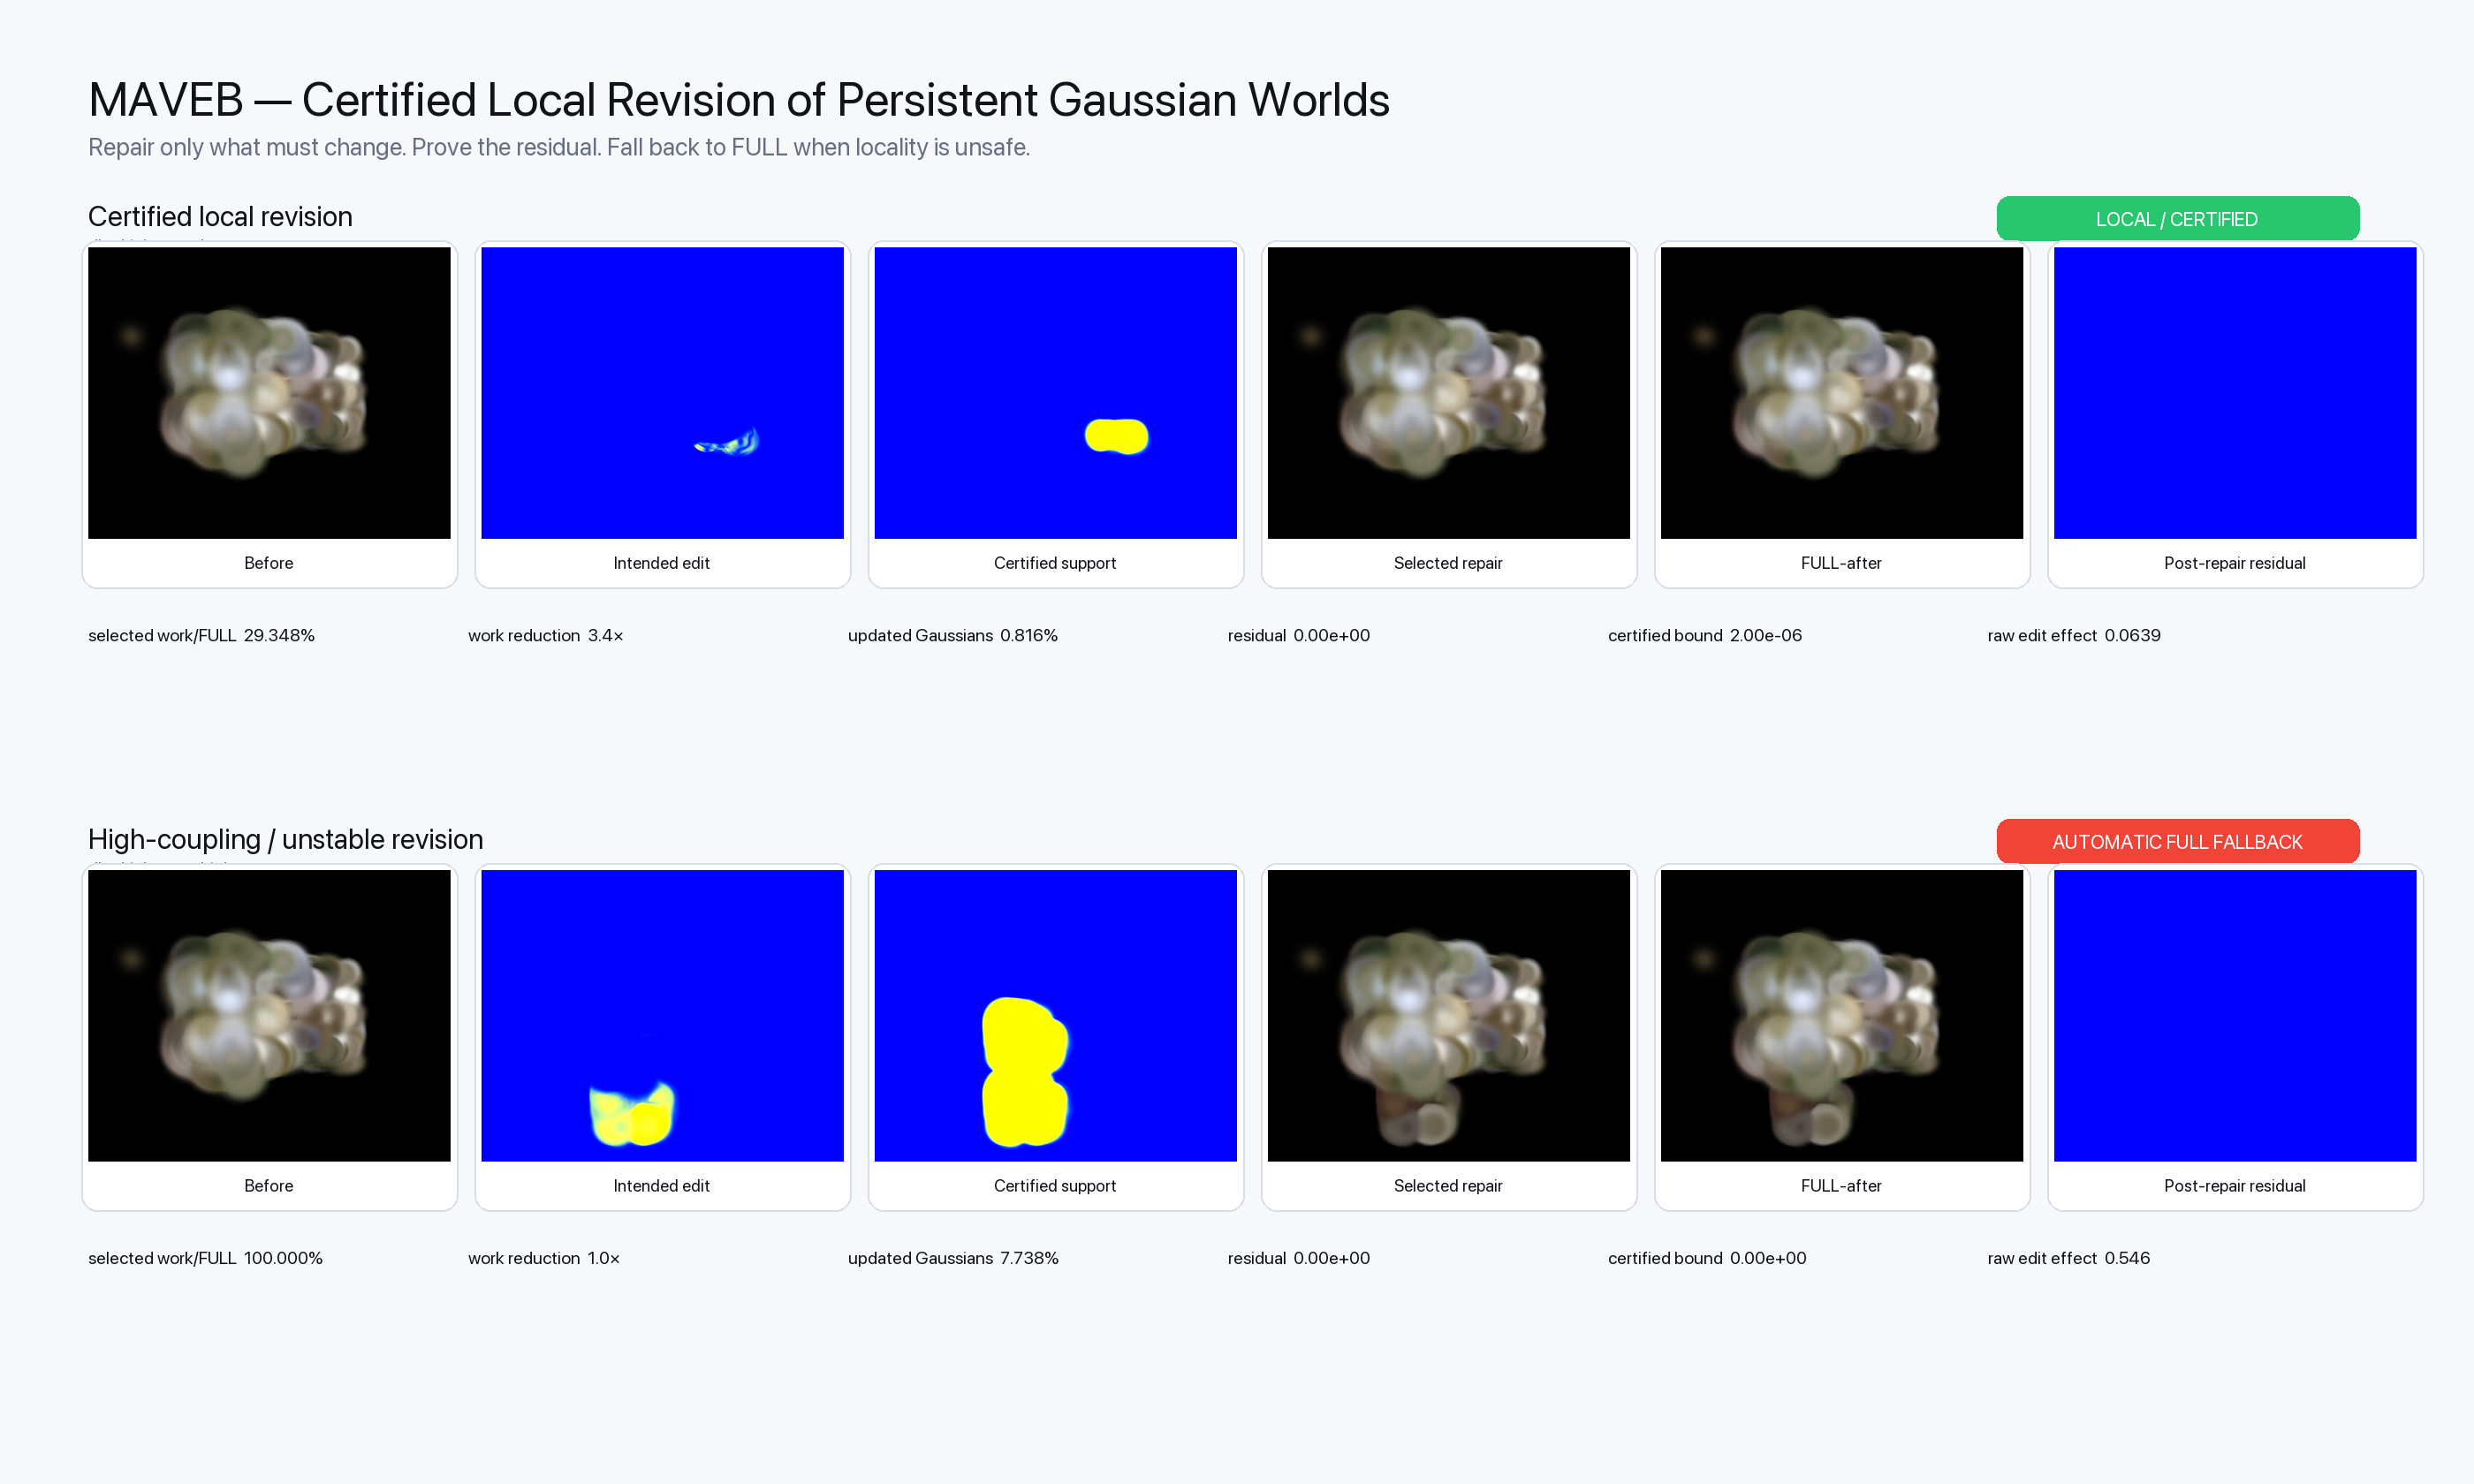
\includegraphics[width=0.95\textwidth]{figures/qualitative_frozen.png}
  \Description{Qualitative frozen MAVEB outcomes. The top row shows a certified local revision with before image, intended edit, certified support, selected repair, full-after reference, and post-repair residual. The bottom row shows a high-coupling revision that falls back to a full rebuild.}
  \caption{Representative frozen revision outcomes. Top: a certified local case repairs only the selected support and matches the independent \FULL{}-after reference at the reported precision. Bottom: a higher-coupling revision expands to an automatic \FULL{} fallback rather than forcing a local decision. The intended-edit and certified-support panels make the source effect and selected scope explicit; the residual panel is computed against the independent full-after oracle.}
  \label{fig:qualitative}
\end{figure*}


\begin{table}[H]
\caption{Canonical evidence summary. Work factors are not wall-clock speedups.}
\label{tab:summary}
\centering
\footnotesize
\rowcolors{2}{gray!8}{white}
\begin{tabularx}{\columnwidth}{@{}Yrr@{}}
\toprule
 & Public RGB/SfM & Trained 3DGS \\
\midrule
Cases & 60 & 5 \\
Certified local & 44 & 4 \\
FULL fallback & 16 & 1 \\
Observed violations & 0 & 0 \\
Selected work / FULL & 0.36953 & 0.03495$^\dagger$ \\
Reported reduction & 2.706$\times$ & 28.614$\times$$^\dagger$ \\
Median inspection / FULL & $\approx1.0$ & 0.999997 \\
\bottomrule
\end{tabularx}
\par\smallskip
\begin{minipage}{\columnwidth}
\footnotesize $^\dagger$Trained results use native temporal/output work, not the public calibrated model. Ratios and reduction factors are medians.
\end{minipage}
\end{table}

\subsection{Trained-3DGS representation check}
The secondary validation uses a pinned public trained 3DGS PLY with spherical-harmonic coefficients, opacity, anisotropic scale, and rotation preserved. Across five frozen revisions, \method{} selected four certified-local repairs and one full fallback with zero observed violations. The median selected native temporal/output work ratio was 0.03495 of \FULL{}, or approximately 28.614$\times$ lower native work under that work definition.

The domain decomposition in Table~\ref{tab:trained} is more informative than the scalar. Median Gaussian update and GPU publication ratios are approximately 0.0182, and temporal invalidation is approximately 0.03495, but Gaussian inspection remains 0.999997 of \FULL{}. Thus the selected update can be highly local while discovery remains essentially global. We treat this as the principal systems limitation of the frozen end-to-end implementation.

\begin{table}[H]
\caption{Median native-domain ratios in the trained-3DGS validation.}
\label{tab:trained}
\centering
\footnotesize
\rowcolors{2}{gray!8}{white}
\begin{tabularx}{\columnwidth}{@{}Y>{\raggedleft\arraybackslash}p{0.24\columnwidth}@{}}
\toprule
\tbhead{Native domain} & \tbhead{Ratio / \FULL{}} \\
\midrule
Gaussian inspection & 0.999997 \\
Gaussian update & 0.018154 \\
GPU publication bytes & 0.018154 \\
Temporal pixels invalidated & 0.034948 \\
\bottomrule
\end{tabularx}
\vspace{3pt}
\caption*{Inspection remains nearly global even when the selected update, publication, and temporal domains are local. The table exposes rather than hides the discovery bottleneck.}
\end{table}

\subsection{Sparse candidate discovery}
A separate exact sparse-discovery sweep tests whether the near-full inspection requirement is intrinsic to candidate selection. Across the sweep, sparse discovery preserves exact candidate-selection agreement while reducing the median inspected fraction to 0.01 and the minimum to 0.001 through the tested scale of up to one million Gaussians (Table~\ref{tab:sparse}). This result demonstrates that the discovery bottleneck is removable in isolation, but it is not silently credited to the frozen end-to-end work ledger because that index was evaluated separately.

\begin{table}[H]
\caption{Separate sparse-discovery study summary.}
\label{tab:sparse}
\centering
\footnotesize
\rowcolors{2}{gray!8}{white}
\begin{tabularx}{\columnwidth}{@{}Y>{\raggedleft\arraybackslash}p{0.34\columnwidth}@{}}
\toprule
\tbhead{Statistic} & \tbhead{Value} \\
\midrule
Exact candidate-selection agreement & true \\
Median inspected fraction & 0.010 \\
Minimum inspected fraction & 0.001 \\
Largest tested scale & 1,000,000 Gaussians \\
\bottomrule
\end{tabularx}
\vspace{3pt}
\caption*{The exact sparse-discovery sweep preserves candidate selection while substantially reducing inspected support. These savings are reported separately and are not credited to the frozen end-to-end headline work number.}
\end{table}

\subsection{Empirical scheduling and ablations}
The held-out changed-fraction scheduler produced no observed unsafe false-local decision on the frozen matrix. This is not evidence that empirical sensitivity is a general safety mechanism: the candidate full-reference residual is zero across these cases, so the matrix does not strongly separate empirical scheduling from certification. \method{} therefore keeps empirical edges outside the certificate by construction.

Table~\ref{tab:ablations} makes the real-matrix ablation behavior explicit. Five structural/analytic ablations are neutral on these 60 cases. The global-norm-tail replacement remains certificate-safe but collapses to \FULL{} on every case. Removing fallback has the opposite failure mode: it never selects \FULL{} and only 26.7\% of cases pass the certificate. The separately labeled mechanism-isolation suite contains seven deterministic synthetic stress cases, one for each v1 mechanism, and all seven separate in the expected safety/work direction. Those stress cases establish falsifiability of the mechanisms, not real-world effect size.

\begin{table*}[!t]
\caption{Frozen real-matrix ablations and their deterministic mechanism-isolation interpretation. Native work ratios use the baseline-suite metric. Neutral means the real matrix matches \method{} on the reported aggregate fields; it is not claimed as evidence that the removed mechanism is unnecessary.}
\label{tab:ablations}
\centering
\footnotesize
\rowcolors{2}{gray!8}{white}
\begin{tabularx}{\textwidth}{@{}>{\raggedright\arraybackslash}p{0.26\textwidth}rrrY@{}}
\toprule
Ablation & Pass & \FULL{} rate & \shortstack{Median native\\work/\FULL{}} & Reading \\
\midrule
Remove predecessor closure & 100.0\% & 26.7\% & 0.04736 & neutral on real matrix; synthetic case exposes omitted required exact work \\
Gaussian analytic $\rightarrow$ \hard{} & 100.0\% & 26.7\% & 0.04736 & neutral on real matrix; synthetic case increases required work or forces \FULL{} \\
Temporal analytic $\rightarrow$ \hard{} & 100.0\% & 26.7\% & 0.04736 & neutral on real matrix; synthetic case increases required work or forces \FULL{} \\
Remove QoI specialization & 100.0\% & 26.7\% & 0.04736 & neutral on real matrix; synthetic case requires extra irrelevant work \\
Collapse \hard{}/\analytic{} separation & 100.0\% & 26.7\% & 0.04736 & neutral on real matrix; synthetic case becomes more conservative \\
Global-norm exterior tail & 100.0\% & 100.0\% & 1.00000 & safe but destroys locality on all 60 real cases \\
Remove certified fallback & 26.7\% & 0.0\% & 0.00000 & 44/60 real cases fail certification; synthetic case leaves an unsafe candidate \\
\bottomrule
\end{tabularx}
\end{table*}

The selected public residual is numerically zero in every frozen case at the reported precision, despite 56/60 source edits exceeding tolerance before repair. The real matrix therefore demonstrates selection/fallback correctness but does not estimate certificate tightness under non-zero accepted residual. We use the threshold-crossing mechanism-isolation cases only to show that the analytic machinery can change decisions when stressed; we do not present them as a substitute for real non-zero-residual evidence.

\section{Discussion}
\subsection{What the evidence establishes}
Within the frozen revision domain and stated bound assumptions, the experiment supports three concrete statements. First, the emitted certificate survived independent full-reference replay in every evaluated case. Second, the planner did not force locality: more than one quarter of public revisions crossed to \FULL{}. Third, when a local result was selected, the frozen calibrated model often assigned substantially less work than a full rebuild. These statements are stronger than showing that a changed-region heuristic happens to work on average, but weaker than a formal proof of universal production safety.

The most important distinction is between \emph{certification} and \emph{prediction}. An empirical scheduler may correctly guess that a local update is safe on all available cases, yet it remains unable to justify an unobserved case unless its prediction is converted into a conservative bound with a valid remainder. \method{} therefore uses empirical information only for scheduling. Conversely, an \analytic{} edge may be conservative enough to force \FULL{} frequently; that is a cost of the safety contract, not a correctness failure.

\subsection{Limitations}
\paragraph{Bounds are only as sound as their assumptions.}
Every exact dependency needed to reproduce repaired state must be represented by \hard{} closure, and every \analytic{} edge must be a finite-change upper bound over the declared revision domain. A representation, shader, temporal rule, or ownership change can invalidate previously calibrated metadata. Certificates therefore require versioned bound provenance and regression tests.

\paragraph{Gaussian discovery remains global in the frozen path.}
The most direct implementation limitation is the near-full Gaussian inspection ratio. Sparse discovery shows that exact selection can be achieved with far fewer inspections, but integration into the complete measured pipeline remains future engineering. This limitation prevents interpreting the current local update ratios as end-to-end complexity reduction across all phases.

\paragraph{No wall-clock speedup claim.}
The 2.706$\times$ public figure is calibrated heterogeneous work reduction, and the 28.614$\times$ trained figure is native temporal/output work reduction. Neither is a paired local-versus-full runtime speedup. A future evaluation should perform matched end-to-end timing under identical execution conditions after sparse discovery is integrated.

\paragraph{Greedy search is not globally optimal.}
Equation~\ref{eq:utility} constructs a certified feasible cone but does not prove that no cheaper safe cone exists. Global combinatorial minimum-work optimization is outside the v1 claim.

\paragraph{Analytic cycles fail closed.}
The reference formulation admits the classical resolvent when its assumptions hold, but the native v1 path certifies finite analytic DAG exteriors. Unsupported cycles trigger cone expansion or \FULL{}. General cyclic certification is future work.

\paragraph{Representation and dataset scope.}
The primary public campaign uses normalized RGB/SfM reconstructions seeded into Gaussian fields rather than trained photorealistic 3DGS, and it is not a metric-scale reconstruction benchmark. The trained-3DGS experiment is a secondary representation check with only five revisions. Broader trained-scene evaluation would strengthen generality.

\paragraph{Ablation identifiability.}
Not every mechanism separates on the frozen real matrix. The paper therefore distinguishes real-workload evidence from synthetic mechanism isolation and does not claim that each mechanism contributes measurable benefit in every scene.

\subsection{Implications}
The larger implication is a change in default behavior for persistent captured worlds. A system need not choose between always rebuilding and trusting a local heuristic. If dependencies can be split into exact and conservatively bounded relations, locality can itself become a runtime decision with a falsifiable output contract. This principle extends beyond Gaussian rendering: caches, temporal histories, spatial acceleration structures, compressed representations, and publication buffers can participate so long as their exact or bounded dependency semantics are explicit.

The framework also makes failure scientifically useful. A certificate violation is not averaged into a quality metric; it is retained as a regression target with the revision manifest, graph version, chosen cone, emitted bound, full-reference output, and first violated invariant. This treatment aligns performance evaluation with the correctness burden created by selective recomputation.

\section{Reproducibility and Artifact Scope}
The canonical evidence freeze records workflow run IDs, artifact IDs, Git SHAs, archive hashes, campaign-row hashes, calibration hashes, and the pinned trained-PLY hash. The public source archive is pinned by byte size and SHA-256; the trained PLY is fetched by explicit repository, revision, path, byte size, and SHA-256 and is not redistributed by \system{}. The project repository includes the dense reference implementation, native planner and oracle, public and trained campaign drivers, baseline and ablation suites, sparse-discovery sweep, deterministic paper-artifact generators, and regression tests.

Scene figures retain applicable upstream terms. Original software is licensed under Apache-2.0; original research communication is scoped under CC BY 4.0; third-party rights are recorded separately. For double-blind review, the public repository and author metadata should be replaced by an anonymized frozen supplement consistent with venue policy.

\section{Conclusion}
We presented Criticality-Bounded Revision Cones, where criticality is the worst normalized certificate-to-tolerance ratio for the protected outputs, as a fail-closed method for selective recomputation in persistent captured worlds. \method{} separates exact dependencies from conservative finite-change influence, binds the unrepaired exterior to explicit output tolerances, compares regional work against a full baseline, and independently replays every selected result against a full-after oracle. The frozen public and trained-representation campaigns show that local repair and full fallback can coexist under one auditable contract, while also exposing a near-global discovery bottleneck and the absence of a current wall-clock speedup claim. The central principle is simple: a persistent world should repair locally only when it can justify what it leaves untouched; otherwise it should rebuild.

\bibliographystyle{ACM-Reference-Format}
\bibliography{references}

\end{document}